\documentclass[]{beamer}
 
\usepackage[utf8]{inputenc} 
\usepackage[T1]{fontenc}
\usepackage{lmodern}
\usepackage{graphicx}
\usepackage[french]{babel}
\usepackage{tikz}
\usepackage{listings}
 %\useoutertheme[subsection=false]{smoothbars}


\usetheme{Warsaw}
%\usetheme{Madrid}
%\usetheme{Frankfurt}
\setbeamertemplate{navigation symbols}{\insertframenumber/\,\inserttotalframenumber}

\begin{document}
 %\hspace*{1cm} \insertframenumber\,/\,\inserttotalframenumber
\title[]{Présentation Berger Levrault}
\subtitle[\ldots]{}
%\author[PETITDEMANGE Franck]{PETITDEMANGE Franck}
%\institute[IRISA]{\includegraphics[width=3cm]{img/logo-irisa.png}}
\date{21 mai 2014}
%\setbeamertemplate{footline}[page number]
\begin{frame}
\titlepage
\end{frame}




\section{Méta-modèle}
\begin{frame}
\tableofcontents[currentsection]
\end{frame}
\subsection{Méta-modèle éléments structuration}
\begin{frame}
\frametitle{Méta-modèle éléments structuration}
\begin{figure}
\centering
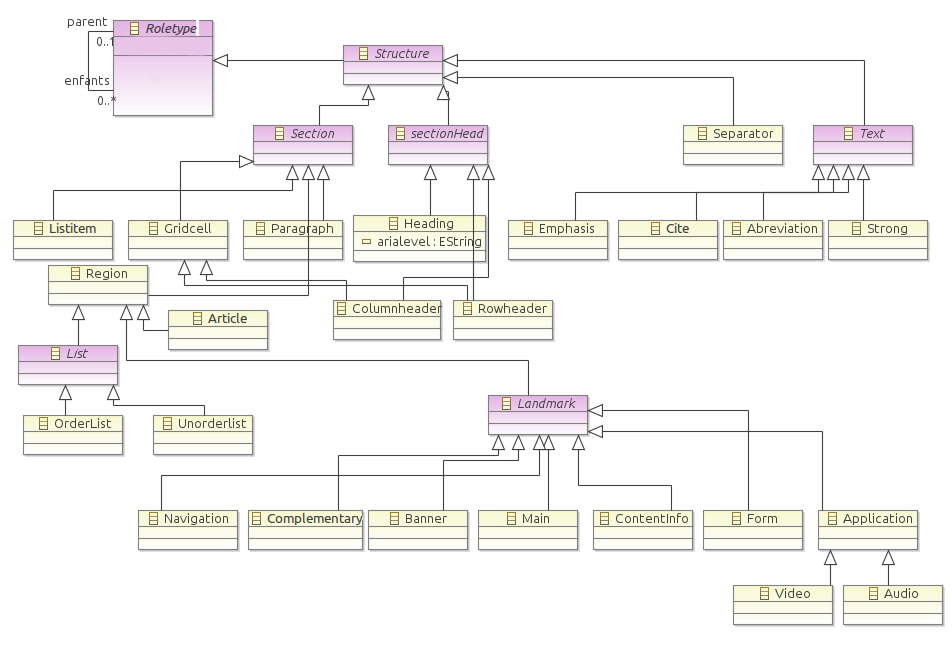
\includegraphics[width=\textwidth]{img/modele-contenu-structure.png}
\end{figure}
\end{frame}

\subsection{Méta-modèle éléments d'interaction}
\begin{frame}
\frametitle{Méta-modèle éléments d'interaction}
\begin{figure}
\centering
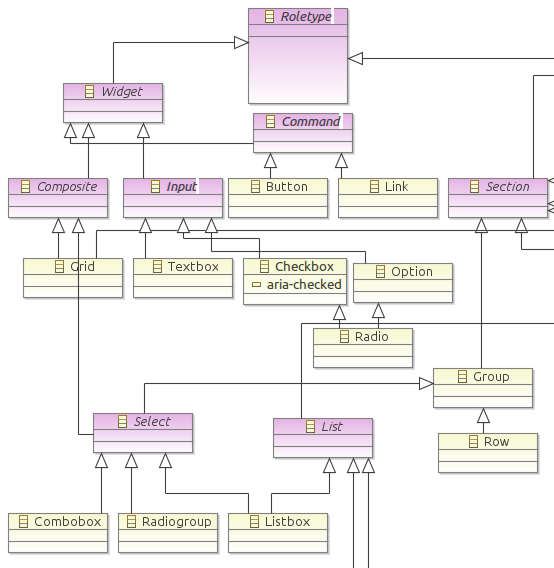
\includegraphics[width=0.5\textwidth]{img/modele-contenu-widget.png}
\end{figure}
\end{frame}

\subsection{Méta-modèle éléments de mise en forme}
\begin{frame}
\frametitle{Méta-modèle éléments de mise en forme}
\begin{figure}
\centering
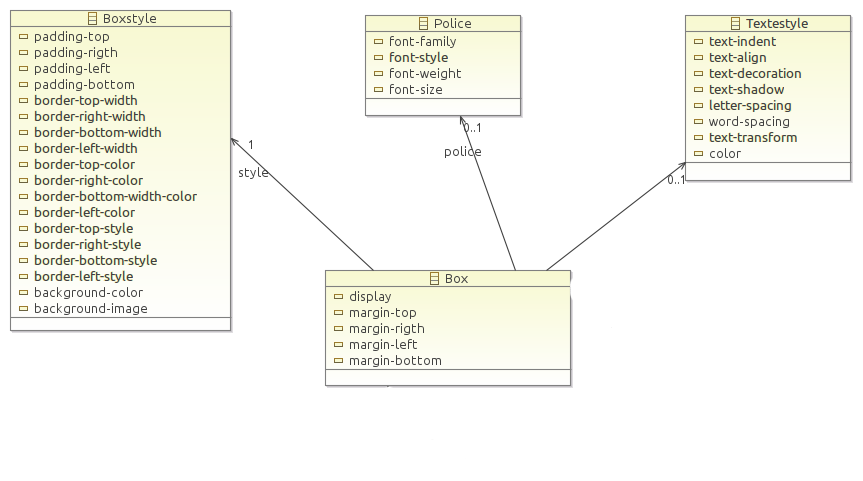
\includegraphics[width=\textwidth]{img/modele-mise-en-forme.png}
\end{figure}
\end{frame}

\subsection{Instance Méta-modèle}
\begin{frame}
\frametitle{Instance méta-modèle}
    \begin{columns}[c] % the "c" option specifies center vertical alignment
    \column{.5\textwidth} % column designated by a command
     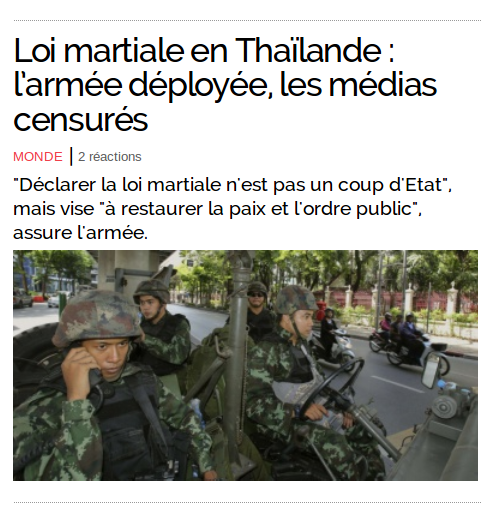
\includegraphics[width=\textwidth]{img/article.png}
    \column{.5\textwidth}
     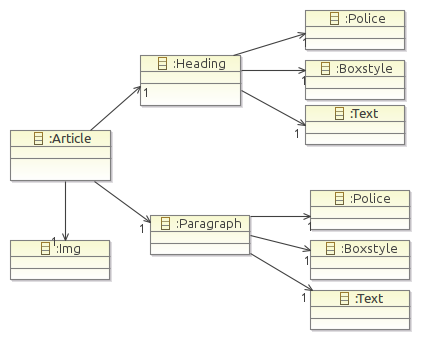
\includegraphics[width=\textwidth]{img/instancearticle.png}
    \end{columns}
    \begin{block}{}
    Article.Heading.Police.fontSize > (Article.Paragraph.Police.fontSize * 1.20)
    Article.Heading.textStyle.color =! "rouge"
	\end{block}
\end{frame}
\section{Extraction structure}

\begin{frame}
\tableofcontents[currentsection]
\end{frame}
\subsection{Démarche générale}
\begin{frame}
\frametitle{Démarche générale}
\begin{figure}
\centering
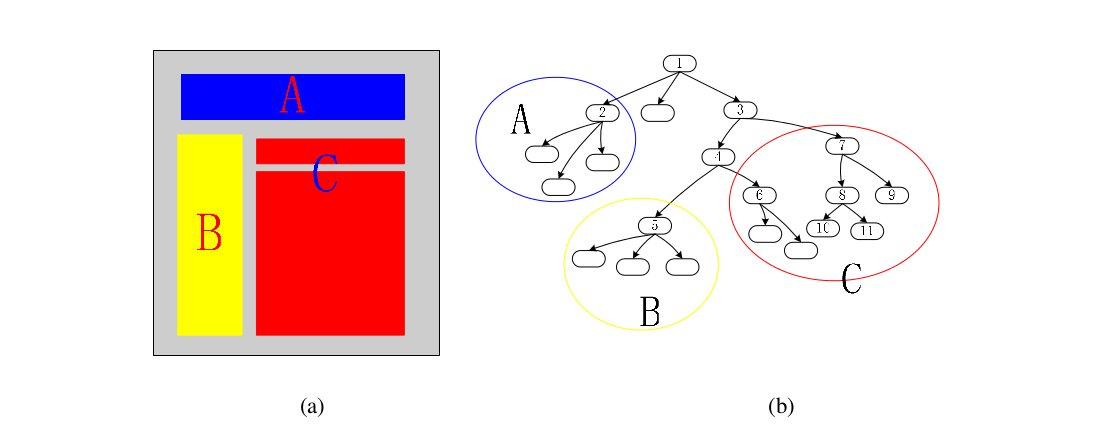
\includegraphics[width=.7\textwidth]{img/VIPS-partionnement.jpg}
\end{figure}
\begin{block}{Approche}
      \begin{itemize}
      	\item Algorithme de segmentation (descendante) basé sur des heuristiques
      	\item Pour chaque bloc extrait (= nœuds non segmentés) est attribué un Degrés de cohérence
      	\item Si le degrés de cohérence est faible alors on ré-applique le processus de segmentation
      \end{itemize}
\end{block}
\end{frame}

\subsection{Heuristiques}
\begin{frame}
\frametitle{Heuristiques}
\begin{itemize}
	\item Informations de mise en forme : 
	\begin{itemize}
		\item nœuds de type\textit{ breakline}
		\item nœuds de type \textit{inline}
		\item nœuds avec des propriétés de couleur
	\end{itemize}
	\item Informations de structuration :
	\begin{itemize}
		\item noeuds avec des tags de structuration <HR>, <P>, <UL>
	\end{itemize}
\end{itemize}

\begin{block}{Exemples d'heuristiques : }
\begin{itemize}
	\item Segmentation des nœuds qui possèdent des enfants de type \textit{breakline}
	\item Extraction des nœuds voisins de <HR>
	\item Division des nœuds dont les enfants ne partagent pas la même propriété de couleur d'arrière plan
\end{itemize}
\end{block}
\end{frame}

\subsection{Résultats}
\begin{frame}
\frametitle{Segmentation étape 0}
\begin{figure}
\centering
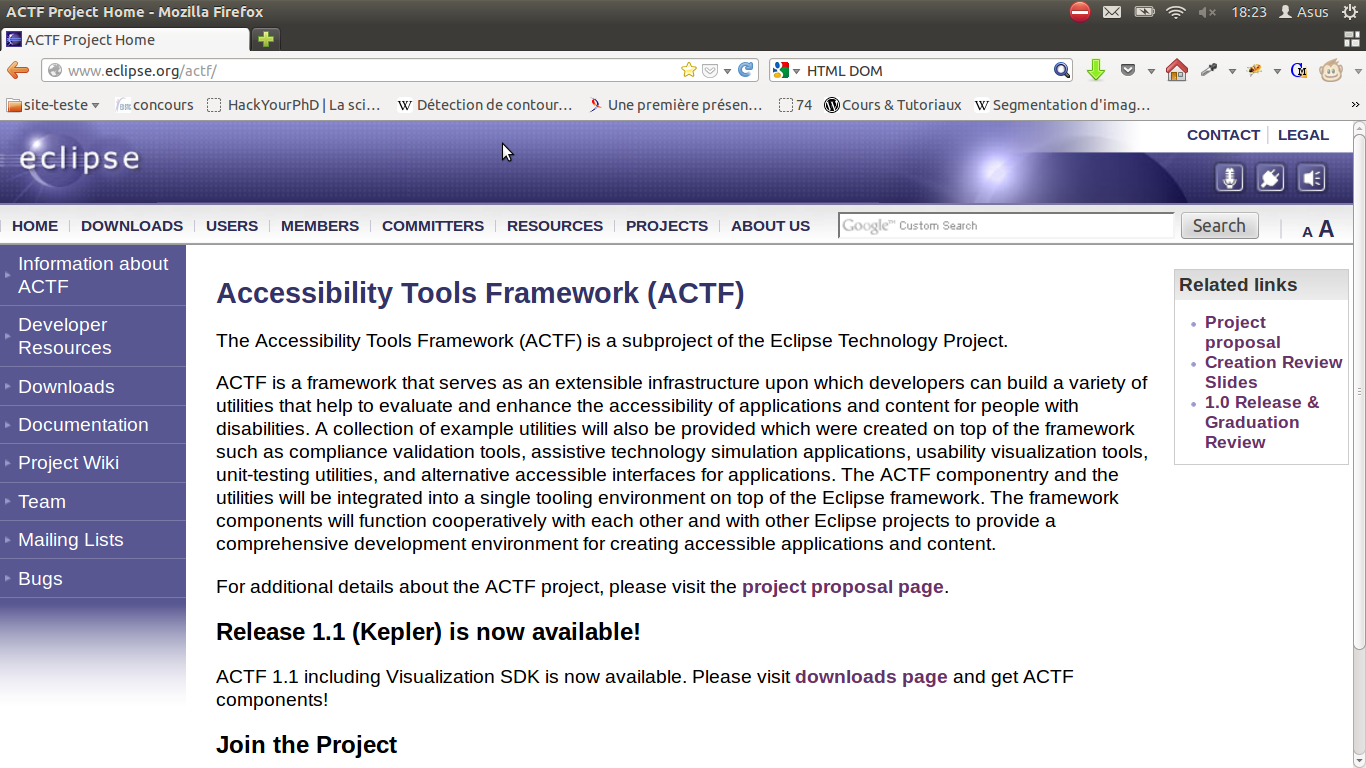
\includegraphics[width=\textwidth]{img/segmentation-etape0.png}
\end{figure}
\end{frame}

\begin{frame}
\frametitle{Segmentation étape 1}
\begin{figure}
\centering
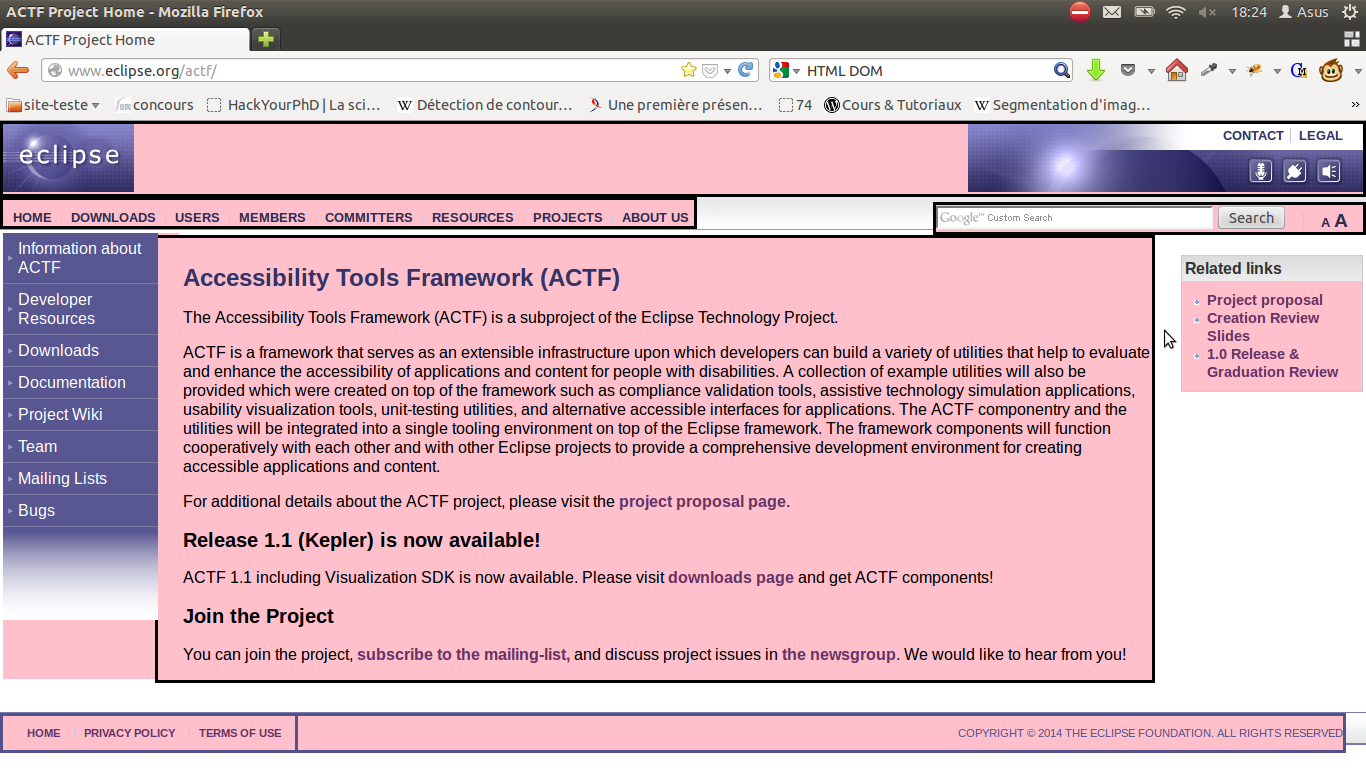
\includegraphics[width=\textwidth]{img/segmentation-etape1.png}
\end{figure}
\end{frame}

\begin{frame}
\frametitle{Segmentation étape 2}
\begin{figure}
\centering
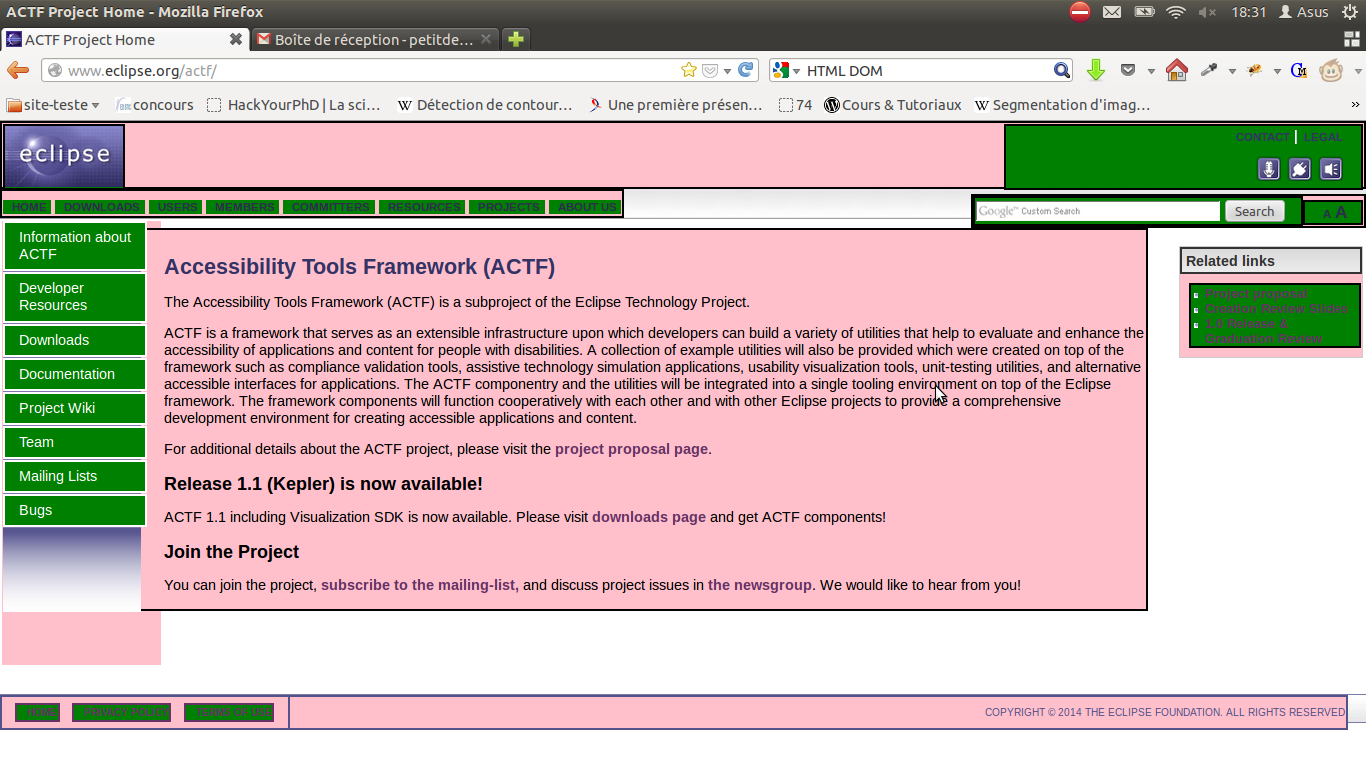
\includegraphics[width=\textwidth]{img/segmenation-etape2.png}
\end{figure}
\end{frame}

\subsection{Difficultés}
\begin{frame}
\frametitle{Segmentation trop souple}
    \begin{columns}[c] % the "c" option specifies center vertical alignment
    \column{.3\textwidth} % column designated by a command
     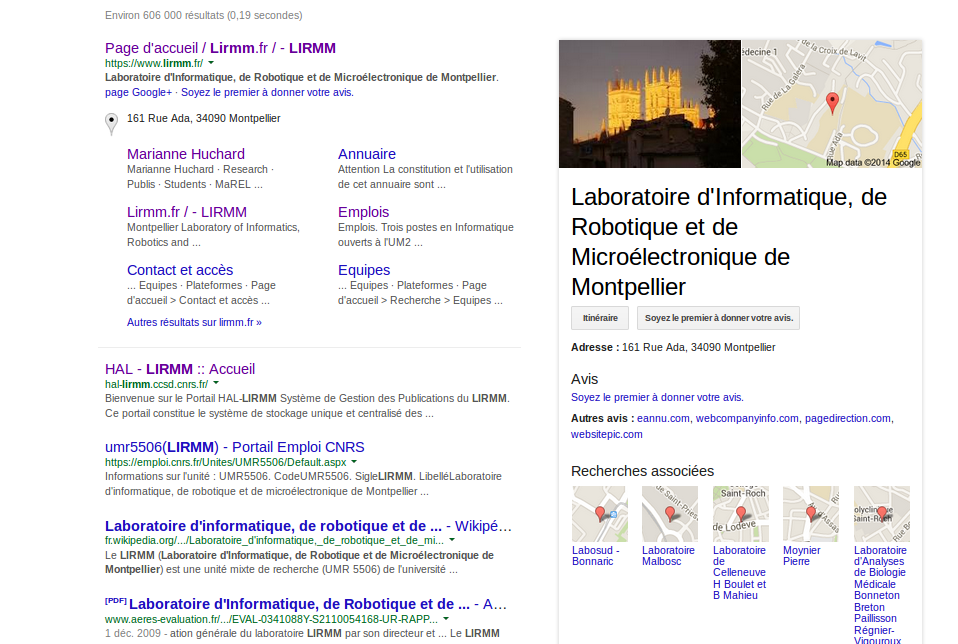
\includegraphics[width=\textwidth]{img/googlesearch.png}
    \column{.7\textwidth}
     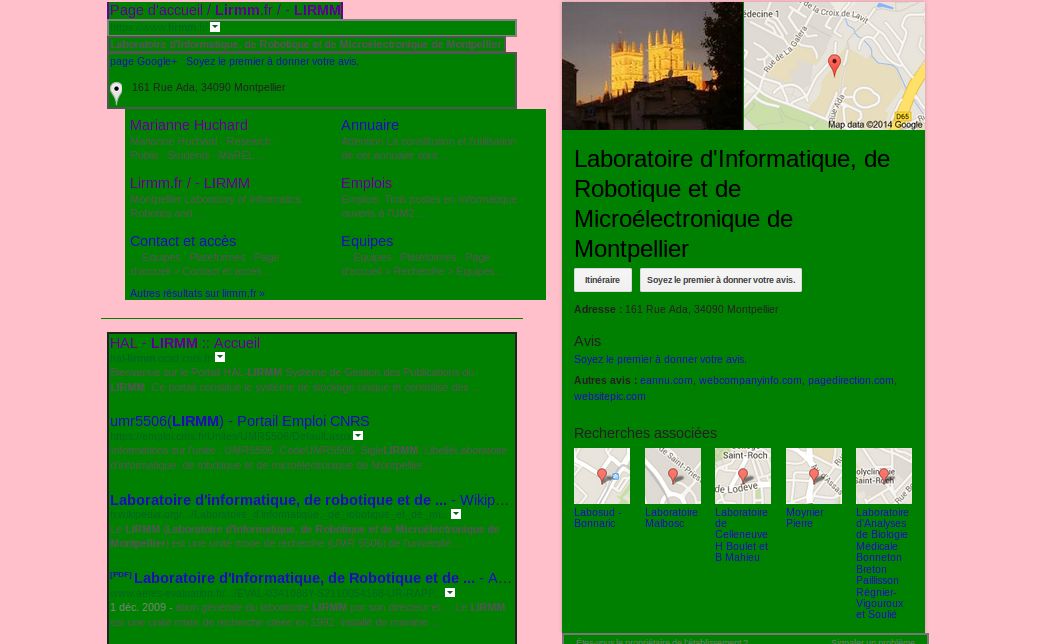
\includegraphics[width=\textwidth]{img/googlesearch-segmentation.png}
    \end{columns}
\end{frame}

%\section{Extraction sémantique}
%\subsection{Les approches}
%\begin{frame}
%\begin{block}{Les approches : }
%\begin{itemize}
%	\item Extraction de la sémantique depuis les balises \textbf{HTML} (uniquement à partir de HTML5)
%	\item Extraction de la sémantique depuis \textbf{CSS} (sémantique connue que par le concepteur)
%	\item Extraction de la sémantique depuis \textbf{RDFa} (standard peu utilisé)
%\end{itemize}
%\end{block}
%\end{frame}


\end{document}
